\chapter{Introduction}
\label{sec:introduction}

The Unbounded Knapsack Problem (UKP) is a simpler variant of the well-known Bounded Knapsack Problem (BKP) and the 0-1 Knapsack Problem (0-1 KP).
The only difference between the UKP and these other KP variants is that the UKP does not impose a bound on the available quantity of each item type.
The UKP can also be seen as a special case of the BKP in which, for each item type, there are more copies available than is possible to fit in the knapsack capacity.

The UKP is NP-Hard and, thus, has no known polynomial-time algorithm for solving it. 
Nevertheless, the UKP can be solved in pseudo-polynomial time by dynamic programming algorithms. 

\section{Motivation and scope}
\label{sec:motivation}

%It's a simpler variant of one of the most classical computer science problems.%,~\cite{pya} (Hybridization between B\&B and DP), and~\cite{DP_inequalities}. % the last is the article from xuequi he, that don't compete with state of the art butonly try new approach
%The UKP has theoretical and applied uses.
%Literature in the area shows many examples of the UKP being used to test solving approaches that were novel at the time as~\cite{mtu1} (Branch-and-Bound) and~\cite{on_equivalent_greenberg} (Consistency Approach).
%Such interest is commonly found in well-known, easy to understand and model, NP-hard problems with practical everyday use, as is the case of the UKP and other KPs.
%Recently, the 0-1 KP has been used to study how humans solve NP-Hard problems~\cite{humans_solve_complex}.
%The author of this thesis finds the use of the UKP (or any other problem) for testing experimental approaches a necessary and relevant line of research.
%However, the author has a critical view about the performance comparison of algorithms over artificial instances that do not model any real-world items distributions.

% CHECAR COM BURIOL
% ``surrogate relaxation of IP problems with non-negative coefficients'' PISINGER p. 147 motivation
%The applied uses of the UKP are related to logistics.
%Also, instances of the BKP or 0-1 KP where there's more copies of each item than ethy can be fit in the knapsack should be solved as UKP, as UKP has some properties that can be exploited for speeding-up the computation that don't exist in BKP and 0-1 KP.

The applied use of the UKP discussed in this thesis is: the UKP as the pricing subproblem generated by solving the continuous relaxation of the set covering formulation for the unidimensional Bin Packing Problem (BPP) and Cutting Stock Problem (CSP) using the column generation approach.
The BPP and the CSP are classical problems in the area of operations research and of great importance for the industry, see~\cite{survey2014} and~\cite{gg-61,gg-63}.
The best lower bounds known for the optimal solution value of the BPP and the CSP are the optimal solution value for their continuous relaxation.
The tightest formulation for the BPP and the CSP has an exponential number of columns and, because of this, is solved by using the column generation approach~\cite{gg-61}.
The UKP is the pricing subproblem of this column generation approach.

%The lower bound provided by the continuous relaxation of those two minimization problems is so tight that it has been speculated that \emph{rounding-up the relaxation optimal value would always give the optimal value of the original problem}~\cite{survey2014}.
%The BPP and CSP instances for which the previous statement is true, are said to have the Integer Round-Up Property (IRUP).
%The conjecture that all BPP and CSP instances had the IRUP property was proven false.
%It is relevant to note that such conjecture was proven false by generating artificial non-IRUP instances, not by finding real-world instances without the IRUP property.
%Also, to the author's knowledge, no BPP or CSP instance proved false the conjecture that all BPP and CSP instances have the Modified Integer Round-Up Property (MIRUP).
%If an instance of the BPP or CSP has the MIRUP, the rounding-up of the relaxation's optimal value will be, at maximum, one unity smaller than the optimal value of the original problem~\cite{survey2014}.

The author of this thesis is aware of the existence of many very good heuristics and approximations for solving the UKP, including the existence of fully polynomial time approximation schemes (FPTAS) for the UKP.
This thesis, however, will only discuss exact methods.
This was done in order to limit scope of this thesis and also because the pricing subproblem instances have to be solved exactly to guarantee that the relaxation is being solved exactly (which in turn guarantee that a branch-and-bound algorithm using the relaxation as a lower bound solves the original BPP/CSP instance exactly).
%if the relaxation is not solved exactly, a branch-and-bound (B\&B) algorithm that used the relaxation as a lower bound would not be exact either.
%While this thesis focuses on the study of the exact algorithms proposed in the literature, and on the instance datasets used to compare them, it also addresses the UKP in the context of the CSP and BPP problems.

%The IRUP and MIRUP properties are defined in terms of the optimal value returned by solving the continuous relaxation of BPP and CSP with an exact method.
%The use of an approximation or a heuristic to solve the pricing problem would make the relaxation solving not exact.
%A study of the effects of using an approximation algorithm to solve the pricing problem would be interesting, but it is not in the scope of this work.

\section{Formulation and notation}
\label{sec:formulation}

%Say solution is a multiset, will be used in the dominance section below
%Say that we consider items with the same weight and profit the same item

The notation presented in this section will be used in the rest of this work.
An instance of the UKP is a pair of a capacity~\(c\) and a list of~\(n\) items.
Each item can be referenced by its index in the item list~\(i \in \{1\dots n\}\).
Each item~\(i\) has a weight value~\(w_i\), and a profit value~\(p_i\).
A solution is an item multiset (i.e, a set that allows multiple copies of the same element).
The sum of the items weight, or profit value, of a solution~\(s\) is denoted by~\(w_s\), or~\(p_s\); and will be referred to as the weight, or profit, of the solution.
A solution~\(s\) is a valid solution iff~\(w_s \leq c\).
An optimal solution~\(s^*\) is a valid solution with the greatest profit among all valid solutions.

To solve an instance of the UKP is to find an optimal solution for that instance.
Finding all optimal solutions for an instance of the UKP is not the focus of this work.
% However, the existence of multiple optimal solutions and the effects of this fact are fully acknowledged. % Marcus Ritt has found five problems in this single phrase.
%We refer to the profit value shared among all optimal solutions for a capacity~\(y\) as~\(opt(y)\), if we omit the capacity then~\(c\) is implied.

The mathematical formulation of UKP is:

\begin{align}
  \mbox{maximize} &\sum_{i=1}^n p_i x_i\label{eq:objfun}\\
\mbox{subject~to} &\sum_{i=1}^n w_i x_i \leq c\label{eq:capcons},\\
            &x_i \in \mathbb{N}_0.\label{eq:x_integer}
\end{align}

%\footnote{If the quantities weren't restricted to the integers the problem wouldn't be NP-Hard.}
The quantities of each item~\(i\) in an optimal solution are denoted by~\(x_i\), and are restricted to the non-negative integers, as~\eqref{eq:x_integer} indicates. 
We assume that the capacity~\(c\), the quantity of items~\(n\) and the weights of the items~\(w_i\) are positive integers. 
The profit values of the items~\(p_i\) are positive real numbers.

%\footnote{If the efficiencies tie the best item is the item with the lowest weight between the tied items.}
The terms \emph{item} and \emph{item type} mean two different things in this work.  The term \emph{item} will be used to refer to an specific item that has a position in the items list of an instance, and that can have duplicates in the same instance.
The term \emph{item type} will be used to refer to a pair of weight and profit value that can be shared by many items.

The efficiency of an item~\(i\) is its profit-to-weight ratio (\(\frac{p_i}{w_i}\)), and is denoted by~\(e_i\). 
We use~\(w_{min}\), or~\(w_{max}\), to denote the smallest items weight, or the largest items weight, within an instance of the UKP.
We refer to the item with greatest efficiency among all items of an specific instance as the \emph{best item} (or simply~\(b\)); if more than one item shares the greatest efficiency, then the item with the lowest weight among them will be considered the best item type; if more than an item has both previously stated characteristics, then the first item with both characteristics in the items list is the best item.
%Also, the item type with the lowest weight among all item types will be refered as the \emph{smallest item}.

%If two or more items have the same weight, we ignore all but the one with the best profit (the others can be discarded without loss to the optimal solution value). The analogue is valid for items with the same profit. Consequently, any two distinct items will always have different weight and profit (only their efficiency can be the same). Items that share the same weight (or profit) can be removed by sorting (\(O(n \times log(n))\)). Ignoring such items simplify the proofs, and don't change the UKP significantly.

The attentive reader will note that an UKP instance is defined by a list of items, instead of a set of items, as usual.
Some algorithms sort the items and manipulate their indices.
So having notation to refer to the items indices is convenient.
Also, a set would not allow for identical items (i.e. that share the same item type).
Such duplicated items exist in some instance datasets of the literature, and can affect the solving time of the algorithms.%As we don't allow distinct items with the same weight and profit, the difference between a list and a set, for the problem formulation, is null.

\section{Properties of the UKP}
\label{sec:well_known_prop}

% TODO: remove the well-known
This section presents properties of the UKP that can be exploited to speed-up its solving.
The main point of these properties is that they are only valid if we have available as many copies of each item type as we could need.
Consequently, those properties are always valid for the UKP and generally not valid for other knapsack variants.
Nevertheless, if every item type~\(i\) of an instance of the BKP (or 0-1 KP) has at least~\(\floor{\frac{c}{w_i}}\) copies available, then the instance can be solved as if it were an instance of the UKP.

\subsection{Dominance relations}
\label{sec:dom_rel}

If one item~\(i\) has the same or less weight than another item~\(j\) (\(w_i \leq w_j\)), and~\(i\) also has the same or more profit value than item~\(j\) (\(p_i \geq p_j\)), then it is clear that if we replace~\(j\) by~\(i\) in any valid solution, the solution will remain valid (the weight of the solution can only remain the same or decrease), as for the profit value of the solution, it can only remain the same or increase.
This relationship between~\(i\) and~\(j\) is called a dominance relation; more specifically, it is a case of simple dominance, in which~\(i\) simple dominates~\(j\). %It's important to note that, as UKP don't limit the quantity of each item type in a solution, we can always do these replacements (what's not true for other KP variants).

We will assume that~\(i\) dominates~\(j\).
There are only two possibilities: the profit value of~\(i\) is greater than the profit value of~\(j\); or they are the same.
If it is the former, then~\(j\) cannot be part of an optimal solution.
By definition, an optimal solution is a valid solution with the greatest profit value; if~\(j\) was part of an optimal solution, replacing~\(j\) by~\(i\) would give a valid solution with an even greater profit value (\emph{reductio ad absurdum}).
If it is the latter (i.e.~\(i\) and~\(j\) have the same profit value),~\(j\) can be part of an optimal solution.
However, we would get an optimal solution with the same or less weight, by replacing~\(j\) by~\(i\) in the optimal solution.

%by an algorithm specific for dominance detection,
If we are interested in obtaining one optimal solution, but not all optimal solutions, we can use dominance relations to reduce the computational effort needed to find a solution.
This is done by detecting dominance relations, and removing the dominated items, thus reducing the size of the problem.
The detection can be done in a preprocessing phase
or within the solving algorithm (reusing computation that would be needed anyway).
% Both approaches have upsides and downsides, some of them will be discussed further in this work.

Dominance relations are not restricted to one single item simple dominating another single item. %can also be applied to solution, instead of single items, and this makes them considerably more interesting.
An item multiset (or solution\footnote{
In this thesis, the term \emph{solution} is used as an synonym for `item multiset'.
A solution does not need to be valid, or optimal (these qualifiers would be meaningless otherwise), and surely does not need to fill the knapsack capacity in a way that no more items can be added to it. 
As the UKP does not limit the quantity of each item type in a solution, we can treat any solution as a new item type, with weight and profit value equal to the weight and profit value of the solution.
}) can dominate a single item too.
Given a solution~\(s\) containing only two or more copies of an item \(i\), and an item \(j\), if \(w_s \leq w_j\) and \(p_s \geq p_j\), then it is said that item \(i\) multiple dominates item \(j\).
This dominance relation is called \emph{multiple dominance}.
Given a solution~\(s\) composed of any items, and an item \(j\), if \(w_s \leq w_j\) and \(p_s \geq p_j\), then it is said that solution \(s\) collective dominates item \(j\).
This dominance relation is called \emph{collective dominance}.
In multiple and collective dominance, whenever we would use item~\(j\) in a solution, we can use the items that constitute~\(s\) in place of~\(j\).
Simple and multiple dominance are special cases of the collective dominance.
Simple dominance can also be seen as a special case of multiple dominance, and some authors use `multiple dominance' to refer to both simple and multiple dominances~\cite{pya}.

\begin{figure}
  \centering
  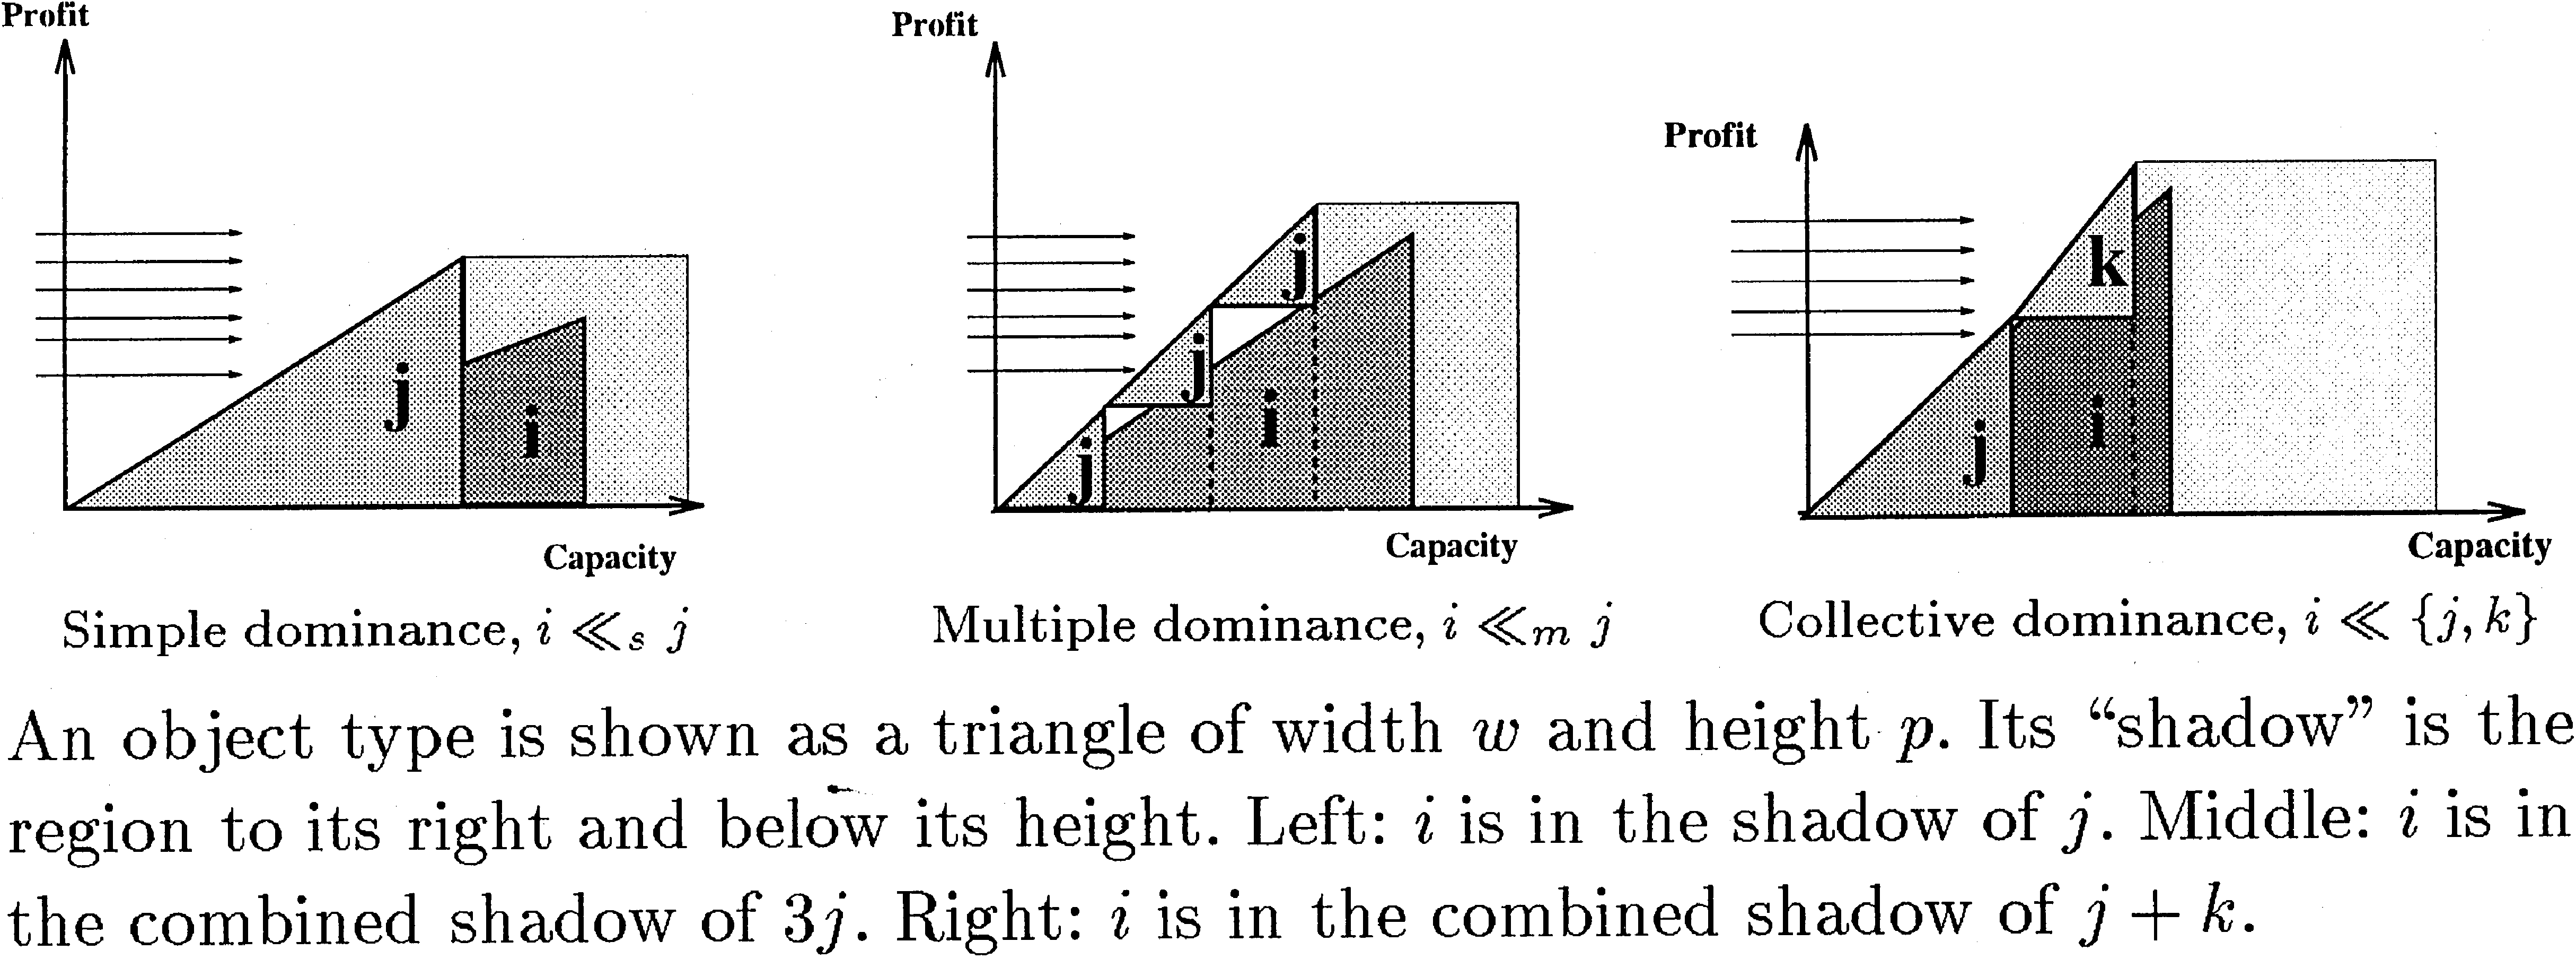
\includegraphics[width=1\textwidth]{smc_dominance}
  \caption{Classical graphic representation of the simple, multiple and threshold dominances. Source: \cite{eduk}. It is interesting to note that the triangle slope equals to the items efficiency, and that all points in the shaded area created by an item or solution triangle are dominated.}
\end{figure}

Given a solution~\(s\) composed of any items, and a solution \(t\) containing only two or more copies of an item \(j\), if \(w_s \leq w_t\) and \(p_s \geq p_t\), then it is said that solution \(s\) threshold dominates item \(j\).
This dominance relation is called \emph{threshold dominance}.
If~\(t\) is composed of~\(n\) copies of item~\(j\), then we know that we can disregard solutions with~\(n\) or more copies of item~\(j\) (as each group of~\(n\) copies of~\(j\) can be replaced by~\(s\) without loss to the value of the optimal solution).
Collective dominance can be seen as a special case of threshold dominance, where~\(n = 1\) (i.e. the dominated solution~\(t\) is a single item solution).

\begin{figure}
  \centering
  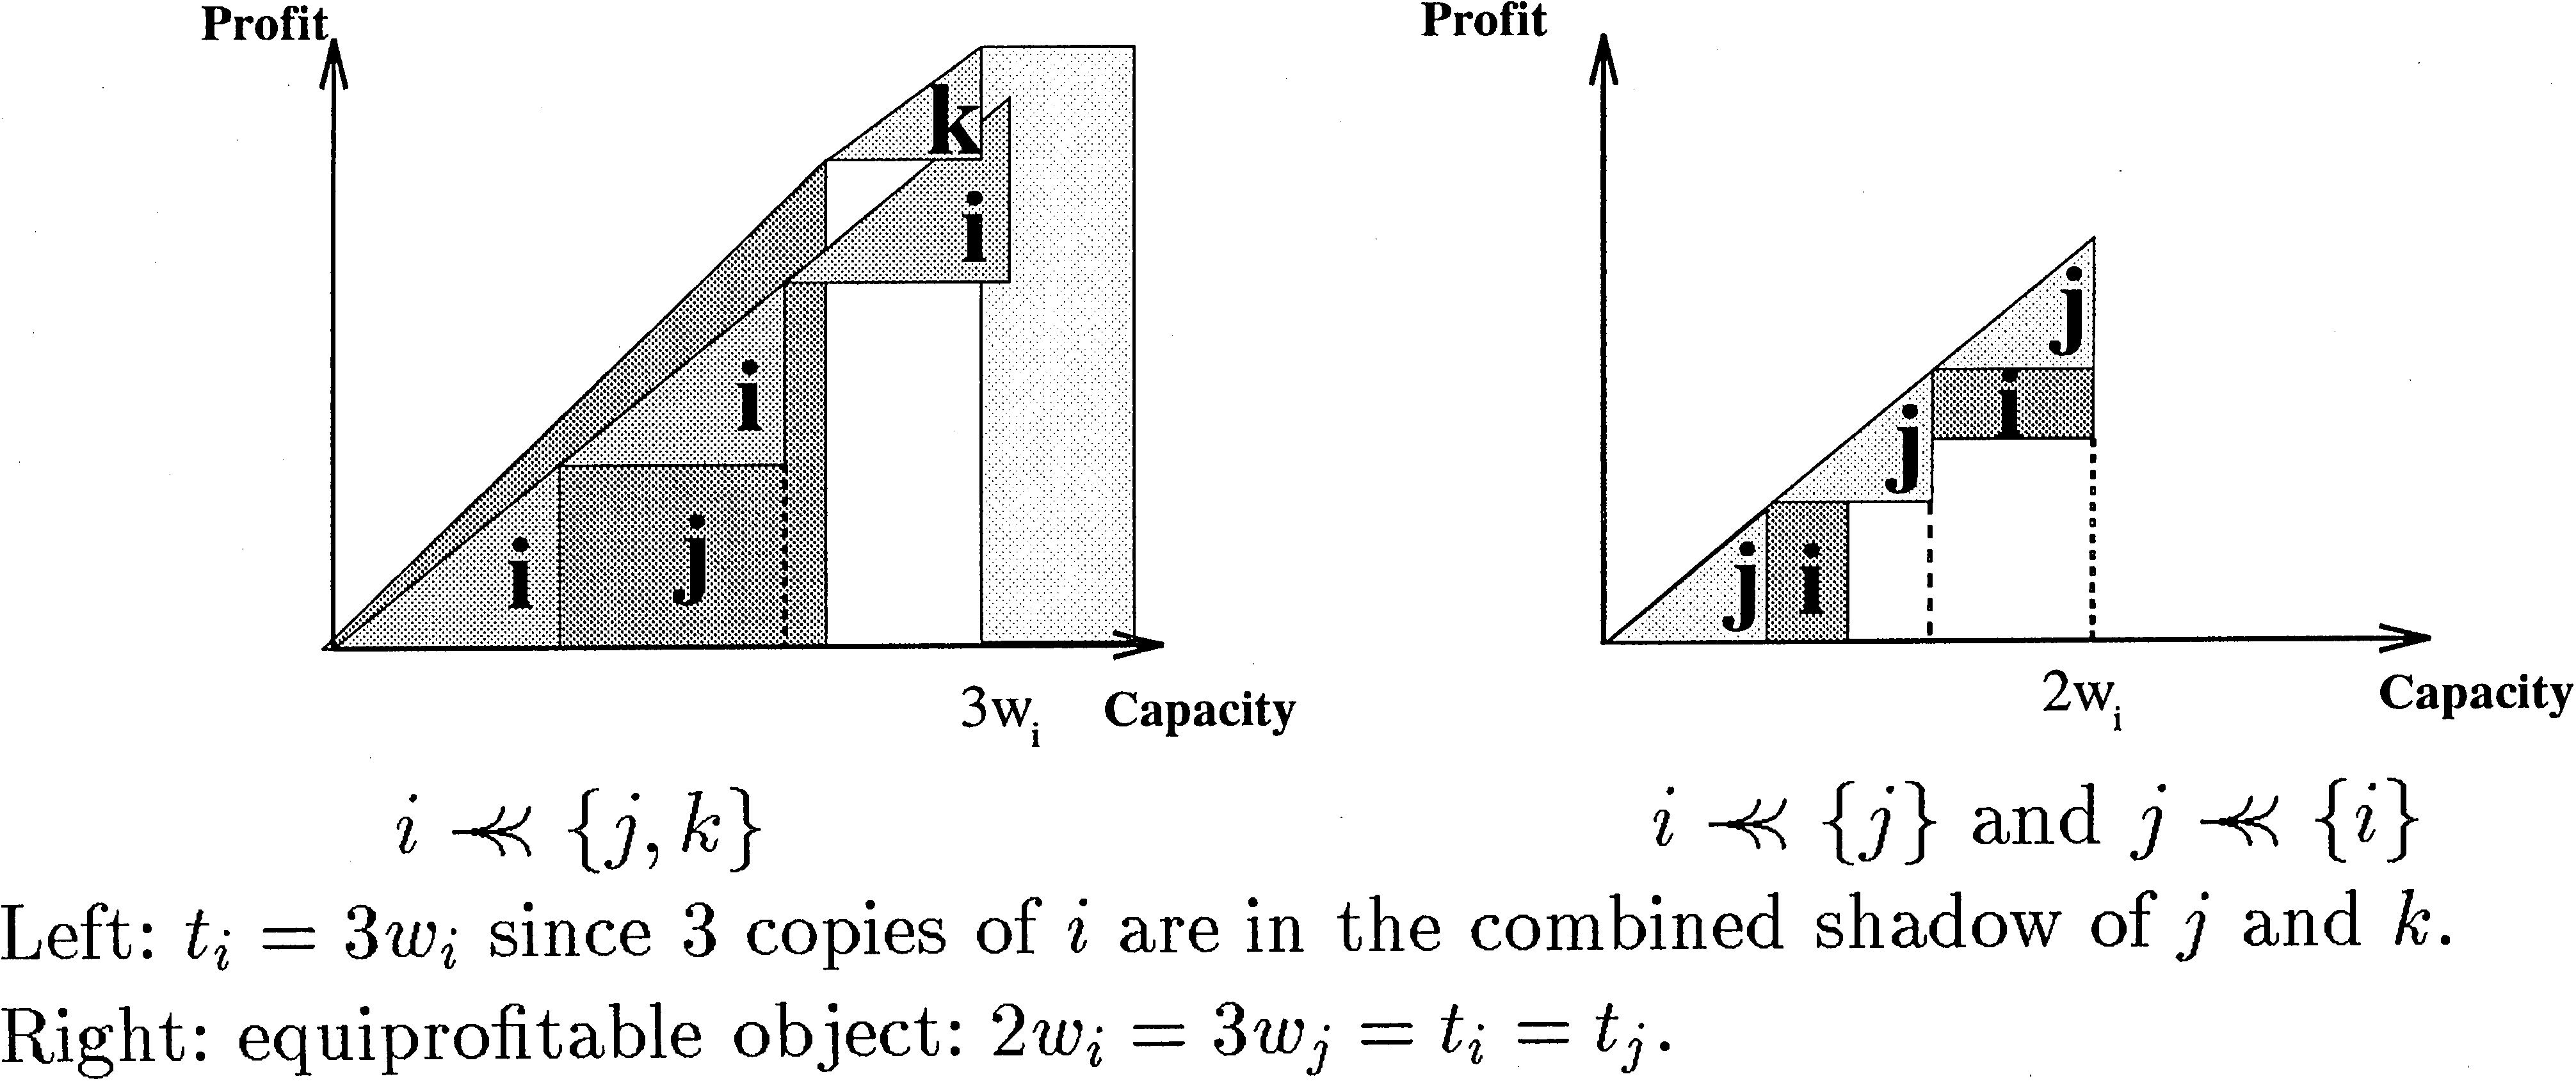
\includegraphics[width=1\textwidth]{threshold_dominance}
  \caption{Classical graphic representation of the threshold dominance. Source: \cite{eduk}. The \(t_i\) is the \emph{t}hreshold of item \(i\), i.e. the weight of the smallest solution composed only of copies of \(i\) that is dominated by another item/solution.}
\end{figure}

The simple and multiple dominances were deeply studied in the previous literature. 
Algorithms that remove all simple and multiple dominated items in~\(O(n^2)\), and heuristics with less complexity that do not guarantee removing all simple or multiple dominated items, were proposed, see~\cite{pisinger_thesis} for a good review on this subject.
On the other hand, the collective and threshold dominances seem too computationally expensive to be done in a preprocessing phase.
However, in the context of a Dynamic Programming (DP) algorithm, in which the optimal solutions of lower capacities can be reused to detect both collective and threshold dominances~\cite{pya}, these dominances are cheap to detect.

The Efficient Dynamic programming for the Unbounded Knapsack problem (EDUK) and the EDUK2 algorithms detect those four types of dominance relations~\cite{pya}.
In fact, threshold dominance was first proposed by the EDUK authors in~\cite{ukp_new_results}, and was a primary feature of the EDUK algorithm.
However, we will see that both algorithms seem to be dominated by algorithms that predate them by about forty years, as the \emph{ordered step-off} algorithm from~\cite{gg-66}, and its `improved version' from~\cite{green_improv}.
These two old algorithms did not directly apply any of the four types of dominance.

After examination, it becomes clear that these two old algorithms indirectly apply all four dominances.
By \emph{indirectly}, we means that, in the course of these algorithms execution, they eventually stop using dominated items to create new solutions, and that happens without testing items for each one of the four dominance relations previously explained.%, and then removing the dominated items from a global items list.
The approach used by these old algorithms is focused on solutions, not individual items.
Consequently, it would be more adequate to say that they make use of some sort of \emph{solution dominance}.
Ideally, given a solution~\(s\) and a solution~\(t\) (both \(s\) and \(t\) can be composed of any items), if \(w_s \leq w_t\) and \(p_s \geq p_t\), then an optimized algorithm could not generate any solutions that are a superset of~\(t\) (as the respective supersets of~\(s\) would dominate them anyway) without loss to the value of the optimal solution..
Such dominance relation would generalize all previous dominances, as the dominated items can be seen as single item solutions (or multiple item solutions, in the case of threshold dominance).

Those old algorithms do not apply this ideal solution dominance, but a weaker version of it.
This weaker version of solution dominance does not avoid generating every solution that is a superset from a dominated solution, but it can be implemented with almost no overhead.
As this is algorithm-specific, it will be further discussed in Section~\ref{sec:ukp5_sol_dom_expl}.

In this section, the concept of dominance was introduced by explaining four dominance relations found in the literature and proposing the concept of strong solution dominance.
In the literature, one of the definitions used for dominance is: ``Given an instance of UKP, relative to item types set~\(N\), item type~\(k \in N\) is dominated if the optimal solution value does not change when~\(k\) is removed from~\(N\).''~\cite[p. 100]{martello_book}.
This definition is consistent with simple, multiple, and collective dominance, but not with threshold dominance.
If an item is threshold dominated, it can still be present in all optimal solutions, it only cannot appear \(n\) or more times in all optimal solutions.
Solution dominance is not covered by this definition, as it is item-centric.
Finally, such broad definition of dominance does not give hints on how to design a procedure for removing the dominated items (without solving the instance), differently from the dominance relations.

\subsection{Periodicity and periodicity bounds}
\label{sec:periodicity}

% TODO: change y to y^{+} in the context of the capacity limit
%The UKP has an obvious periodic property that for every knapsack capacity that is a multiple of the best item's weight, the optimal solution for that knapsack capacity is~\(\frac{c}{w_b}\) copies of the best item (it's clearly the most efficient use that can be made of such capacity). The UKP has also a not-so-obvious and more interesting periodic property that states that:
The UKP has an interesting periodic property that can be stated the following way: for every set of item types, there exists a capacity~\(y^+\), for which every capacity~\(y'\) (\(y' > y^+\)) will have an optimal solution that is an optimal solution for capacity~\(y' - w_b\) with one more copy of the best item added.
In other words, after some capacity~\(y^+\), we can find optimal solutions simply by adding copies of the best item to optimal solutions of capacities~\(y^+\) and lower (all other items are not relevant anymore).
In the literature, this periodic property is called \emph{periodicity}.
It should be clear that if we knew~\(y^+\) beforehand, and~\(y^+ < c\), then we can solve the UKP for the capacity~\(y^{*} = c - \ceil{\frac{c - y^+}{w_b}}w_b\) and fill the gap between~\(y^{*}\) and~\(c\) with exactly~\(\frac{c - y^{*}}{w_b}\) copies of the best item (instead of solving the UKP for capacity~\(c\)).
%The focus of this section will be this second periodic property, that we will call simply by `periodicity'.

The periodicity is a direct consequence of the threshold dominance.
However, the periodicity was discovered much before the concept of threshold dominance.
For instance, periodicity was already described in~\cite{gg-66}.
As the concept of threshold dominance was already explained in this thesis, the author will use it to explain periodicity.

The threshold dominance property states that, if a solution~\(s\) dominates solution~\(t\), and~\(t\) contains only~\(n\) copies of the same item type~\(j\), then solutions with~\(n\) or more copies of~\(j\) can be be replaced by solutions using~\(s\) instead (without loss to the value of the optimal solution).
The periodicity property states that after some capacity~\(y^+\) we can obtain optimal solutions only by adding copies of the best item to the optimal solutions from capacities \(y^+\) or below (all other items are not relevant anymore).
The link between these two properties is that \emph{for a sufficiently large capacity, solutions composed of copies of the best item will threshold dominate solutions composed of copies of any other item}.

First, we will verify the truth of the statement above.
For any two positive integers~\(a\) and~\(b\) there will always exist at least one integer number that is divisible by both~\(a\) and~\(b\) (e.g.~\(a \times b\), or their \emph{least common multiple},~\(LCM(a, b)\)).
Therefore, for each non-best item~\(j\), there will exist a capacity value~\(y\) that it is divisible by both~\(w_b\) and~\(w_j\).
Given~\(m_j = \frac{y}{w_b}\) and~\(n_j = \frac{y}{w_j}\), and by the definition of best item, we have that~\(m_j \times p_b \geq n_j \times p_j\).
In other words, a solution composed only of~\(m_j\) copies of the best item will threshold dominate a solution composed only of~\(n_j\) copies of item~\(j\).

It is important to notice that, in the case of an instance in which all items have the same efficiency, the best item (that will have weight~\(w_{min}\) by definition) will threshold dominate each other item at the capacity that is the \emph{lowest common multiple} between their weights (as shown in the last paragraph).
However, if the best item~\(b\) is more efficient than the non-best item~\(j\) (which is more common), then a smaller solution~\(s\) composed only of copies of~\(b\) can be more profitable than a bigger solution~\(t\) composed only of copies of~\(j\).
The weights of the two solutions do not have to be the same.

Now, we explain how periodicity is a direct consequence of threshold dominance.
As we have seen, for each non-best item~\(j\), there will exist a positive integer~\(n_j\), in a way that solutions with~\(n_j\) copies of~\(j\) are dominated by solutions that use~\(m_j\) copies of~\(b\) instead.
We will assume that there exists a solution~\(u\) composed of~\(n_j - 1\) copies of each item~\(j\).
If another copy of any item~\(j\) is added to~\(u\), the resulting solution~\(u' = u~\cup~\{j\}\) could be replaced by another solution~\(v\) that contains no copies of~\(j\), and~\(m_j\) additional copies of~\(b\).
Any solution that weight more than solution~\(u\) has only two possibilities: it uses more copies of the best item; or it uses more than~\(n_j\) copies of some non-best item~\(j\).
In the last case, copies of~\(j\) can be replaced by copies of~\(b\) until the quantity of copies of~\(j\) is smaller than~\(n_j\).
Consequently, after the knapsack capacity~\(y'' = w_u\), adding copies of other items to a solution would be equal to adding copies of the best item (making any other item type except~\(b\) irrelevant).
Note that~\(y''\) is only an \emph{upper bound} on~\(y^+\), the value of~\(y^+\) can be smaller than~\(y''\), as the items that the best item threshold dominate, can themselves threshold dominates other items.

It's worth mentioning that computing the exact value of~\(y^+\) is a very expensive process that equals to solving the UKP for all capacities~\(y^+\) and lower while checking for threshold dominance.
The author do not know any algorithm for solving the UKP that computes the exact value of~\(y^+\) before starting to solve the UKP.
The algorithms compute an \emph{upper bound} on the~\(y^+\) capacity value, as the one presented in the previous paragraph, that was presented in~\cite[p.~215]{book_ukp_2004}.

An upper bound on~\(y^+\) is less valuable than~\(y^+\) itself, but it can be computed in a reasonable polynomial time, before starting the solving process.
If one algorithm checks for threshold dominance periodically, it can stop when all non-best items have been threshold dominated by the best item.
Such algorithm would not benefit much from computing an upper bound on the~\(y\) capacity value.
If this algorithm setup phase (e.g. allocating and initializing memory) is linear in the knapsack capacity~\(c\) and the upper bound on the~\(y\) capacity value is considerably smaller than \(c\), then the algorithm could benefit from the upper bound. 

There exist many proposed periodicity bounds, but some are time-consuming, as the~\(O(n^2)\) periodicity bound presented in~\cite{badbound1}. Others depend on specific instance characteristics to be tight, as the ones presented in~\cite{badbound2} and~\cite{pya}.
For reasons that will be made clear in the conclusions, the author did not found relevant to present a review on periodicity bounds in this work.
The UKP5 algorithm makes use of one simple periodicity bound, and it will be explained together with UKP5 in Section~\ref{sec:ukp5_periodicity}.

